\chapter{Introduction}
%l
Semantic segmentation is the task of predicting regions across the entire image and is also known as pixel-level segmentation \cite{DBLP:journals/corr/abs-1809-10198semanticprogress}. 
It is known as pixel-level segmentation/accuracy because every pixel of the image is associated with a class. 
Semantic segmentation is a problem where you need not only pixel wise accuracy, but multi-scale context as well \cite{Yu2016MultiScaleCA}. 
This is due to the fact that we need to use the multi-scale context in order to predict correctly at the pixel level. 
For example a horse in an image has many pixels associated with it, but one would need to know what a horse looks like in order to correctly predict each pixel in the image. 
This problem has been discussed extensively for natural images \cite{DBLP:journals/corr/LongSD14}, \cite{DBLP:journals/corr/ChenPSA17}, \cite{Yu2016MultiScaleCA} as well as for medical images \cite{DBLP:journals/corr/RonnebergerFB15}. 
There are many applications for semantic segmentation not only in the medical field, such as for autonomous driving \cite{inbookautomous}, facial segmentation \cite{7350915face} and many other applications. 

The medical field has a great use for autonomous semantic segmentation because segmenting medical images is a time consuming task for doctors.
In order to get a good segmentation a doctor not only needs great expertise in the forming of the regions, but also needs to take the time to manually draw it out, when they are busy with many other tasks.  
Autonomous semantic segmentation will help reduce the time it takes to fully segment a medical image drastically with the doctors only having to spend time to study the image for the patient.
This will also aid doctors not only in the diagnosis of the patient, but also help to standardize the process so that fatigue or human error doesn't affect the results of the segmentation \cite{SharmaAutomatedImageSegmentationTech}. 
This paper will focus on the task of semantic segmentation of the brain, specifically rat brain MRI's.
This paper proposes an implementation of the most popular methods for semantic segmentation and applies it to rat brain MRI's taken over time. 


\subsection{Semantic Segmentation and MRI images}
        Magnetic Resonance Imaging or MRI is a radiology technique that produces three dimensional anatomical images. 
        MRI utilize a strong magnetic field as well as radio waves in order to measure the energy released from atoms realigning with the magnetic field \cite{doi:10.1002/9781118786574.ch1MRI}. 
        Different types of tissue have different magnetic properties and so using the MRI technique we are able to differentiate them within the image. 
        MRI is a type of anatomical imaging where the goal is to create an accurate visual representation of the tissues being imaged. 
        Doctors are able to use MRI images for many purposes, for example to diagnose diseases or to see any abnormalities in a person's body. 
        There also also multiple different sequences for MRI's that correspond to different types of tissue being more excited than others.
        Some of the most common sequences are T1 weighted, T2 weighted, and Flair where each one corresponds to different tissues being excited more than others. 
        This paper will just focus on T2 weighted MRI's.
        MRI of the brain is usually taken in a 3D volume. 
        Each MRI will consist of a x,y, and z dimensions corresponding to a series of 2D images.
        The reason that it can correspond to a series of 2D images is that the voxels in the MRI are not necessarily evenly spaced in different dimensions. 
        Usually the z dimension is differently spaced than the x,y dimensions, but it depends on a number of factors like MRI magnet strength, imaging parameters, etc.
        
\begin{figure}
\centering
\begin{subfigure}{.5\textwidth}
  \centering
  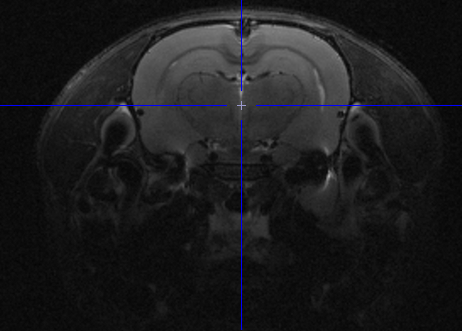
\includegraphics[width=.6\linewidth]{coronal_brain_view.png}
  \caption{Coronal slice of a rat brain}
  \label{fig:coronal}
\end{subfigure}%
\begin{subfigure}{.5\textwidth}
  \centering
  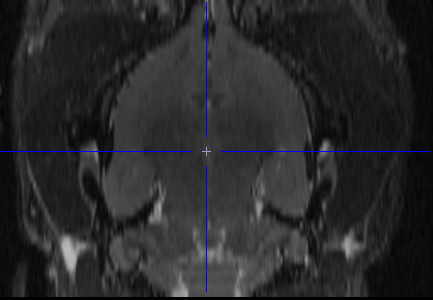
\includegraphics[width=.6\linewidth]{axial_brain_view.png}
  \caption{Axial slice of a rat brain}
  \label{fig:axial}
\end{subfigure}
\begin{subfigure}{.3\textwidth}
  \centering
  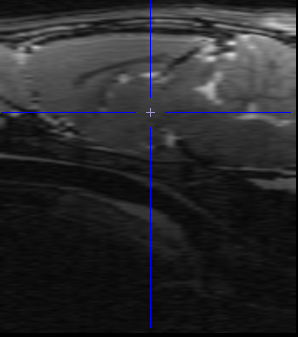
\includegraphics[width=.6\linewidth]{sagittal_brain_view.png}
  \caption{Saggital slice of a rat brain}
  \label{fig:saggital}
\end{subfigure}

\caption{This figure shows an example of the data that will be used in this paper. They are T2 weighted MRI images of size 280x200x44. }
\label{fig:MRI image}
\end{figure}

        
        The data used in this paper is provided by the CMGI or the Center for Molecular or Genome Imaging and consists of rat brain T2 wieghted MR images. 
        The study imaged 40 total different rats at three separate time points; day 3, day 7, day 28. 
        This study was conducted to learn more about the effects of anti-seizure drugs.
        It is important to note that the rats were given Diisopropyl fluorophosphate or DFP to induce seizures. 
        Some rats were also given anti-seizure drugs, Midazolam (MDZ) and Diazepam (DZP) and imaged to compare the effects of the drugs.
        This paper will focus on implementing an autonomous method that can segment multiple regions in MR images. 
        The 40 animals were split up in multiple groups in order to effectively test the drugs.
        The dataset was split into 10 animals for the the control group or vehicles (VEH), 10 animals that are given DFP and basic treatment, 10 animals that are given DFP and then MDZ, and 10 animals that are given DFP and DZP. 
        Each one of these animals had MR images taken at three different time points mentioned above for a total of 120 scans. 
        Each one of these scans was semantically segmented by two people who tried to stay as consistent as possible. 
        The ground truth is segmented into 14 different regions pertaining to areas in the brain and will be explained in more detail later in the paper. 
        
\section{Statement of Problem} 


    Semantic segmentation has been implemented successfully with the invent of deep neural networks.
    The medical field has a great need for semantic segmentation, but the availability for medical images to train on is usually scarce, compared to the thousands or millions of images available in the natural world.
    This makes the task of semantic segmentation much harder when applied to the medical field as when it comes to training deep neural networks data is essential. 
    
    There are many problems associated with segmentation segmentation, especially when it applies to the medical industry. 
    One of the main problems is that models can't be trained with millions of images like in the natural image case. 
    It is very hard to obtain a large data set when it comes to medical images because of privacy laws as well as just general availability of the images. 
    It is much easier to find many different images and its segmentation of a horse than a brain. 
    Before the medical images can be used in models it has to have no connection with the 
    A lot of the time the images being gathered have personal data attached to it and so before the data can be used into a model all information that can be used to identify it has to be removed. 
    
    Another big challenge is that getting the ground truths of the data is very time consuming. 
    In order to be able to accurately segment an image of the animal, one needs to be an expert in that animal. 
    It is not common knowledge to know how to segment the different regions in a brain are versus the segmentation of a horse.
    There are no clear boundaries in some regions of the brain and so a lot of the time experts will segment the regions slightly different. 
    The segmentation will also vary from person to person because some people are more familiar with certain brain regions than others and might have more experience as well as people's brains are different as well.
    
    One of the main challenges using this data for segmentation is that the data provided by the study varies a lot. 
    The VEH or control group stays the most consistent whereas the DFP group after a certain amount of time the brain region even for the same animal will have vastly different segmented regions.  
    This is due to brain loss and other complications due to the induced seizure that the rats go through.  
    
 

\section{Outline}
    This paper will first go more in detail about some of the best ways currently that are used for semantic segmentation which will be in chapter 2. 
    Chapter 3 will be focused on our approach to semantic segmentation issue. 
    Chapter 4 will discuss the data in more detail and how we utilize it in our models. Chapter 5 we will discuss the results and finally in Chapter 6 we will conclude the work of this paper and discuss some options in the future.